\chapter{Planificación y Seguimiento}

En este capítulo detallaramos la planificación de cada una de las iteraciones que hemos hecho, así como el seguimiento realizado. La elaboración de este proyecto se llevó a cabo durante dos años, comenzando en junio de 2014 y teniendo un par de parones durante varios meses (desde septiembre de 2014 hasta enero de 2015 y desde mayo de 2015 hasta septiembre del mismo año). 
Por lo tanto, los periodos de actividad serían los siguientes:

\begin{itemize}
  \item Desde junio del año 2014 hasta septiembre del 2014 (3 meses).
  \item Desde enero de 2015 hasta mayo del mismo año (4 meses).
  \item Desde septiembre del 2015 hasta abril de 2016 (8 meses).
\end{itemize}

En las próximas secciones hablaremos de lo que hemos desarrollado durante estos tres periodos de tiempo y las iteraciones seguidas en los mismos.

Cabe destacar que todos los datos y tareas mostradas a continuación están realizadas de forma lineal, dado que solamente disponemos de un recurso.

\section{Junio 2014 - Septiembre 2014}

Este periodo comienza el 4 de junio, que es cuando se nos comenta la posibilidad de realizar este proyecto, y termina el 24 de septiembre, por lo que consta de un total de 15 semanas. Hay que tener en cuenta que durante parte de este verano (desde agosto) es cuando me mudé a Holanda y empiecé mi \textit{internship}, por lo que las jornadas en días laborables solamente constaban de una o dos horas y alrededor de 8/9 horas durante los fines de semana.

Sumando todo el tiempo empleado durante estas semanas se calcula que se han empleado 190 horas en total.

Durante este tiempo nos centramos en recabar información general para poder empezar el proyecto con buen pie, así como la implementación de los mapas y habitaciones.

\subsection{Primera iteración: Análisis de requisitos generales, diseño genérico y preparación y configuración de los elementos necesarios para el comienzo de la implementación}

Desde el 4 de junio hasta el 29 de junio.

\paragraph{Análisis de requisitos generales} Al desarrollar un proyecto enfocado a una parte de la población de la que no formas parte, es muy importante documentarse sobre todos los aspectos que hay que tener en cuenta e intentar ponerse en su piel (por ejemplo usar las herramientas que utilizan diariamente para recabar ideas).
Àsí mismo, desarrollar un videojuego puede llegar a ser una tarea infinita, dado que nuevas características o ideas que añadir es algo que sucede casi diaremente. Aprender sobre lo básico del género y poner límites es fundamental para centrar los pocos recursos que tenemos en crear lo completamente necesario.

\paragraph{Diseño genérico del juego a implementar} Crearemos el primer diseño genérico que nos dará una idea sobre lo que tendremos que realizar y nos guiará sobre el proceso de creación del juego. Este primer boceto cambiará a medida que querramos añadir nuevos elementos y querramos especificar más otros.

\paragraph{Búsqueda de bibliotecas que se adapten a nuestros requisitos} Hay varias bibliotecas con las que se puede crear una interfaz gráfica sencilla como la de Rogue, pero todas ellas tienen sus ventajas e inconvenientes. Debemos de averiguar cuál de ellas es la más adecuada para nuestro caso.

\paragraph{Creación y configuración del ambiente de desarrollo para poder empezar la implementación} Al empezar un nuevo proyecto debemos de crear un repositorio en git, instalar todo el software necesario y preparar lo básico para que podamos empezar a programar sin encontrarnos con ninguna dificultad a posteriori.

\subsubsection{Tareas y seguimiento}

La descomposición de las tareas es la siguiente:

\begin{enumerate}[label=\bfseries WBS 1.\arabic*]
  \item Análisis de requisitos generales
    \begin{enumerate}[label=\bfseries WBS 1.1.\arabic*]
      \item Estudio de herramientas para invidentes.
      \item Estudio de los elementos del género \textit{roguelike}.
      \item Analizar los elementos encontrados y especificación de lo que queremos en nuestro caso.
    \end{enumerate}
  \item Diseño genérico del juego a implementar.
  \item Búsqueda de bibliotecas que se adapten a nuestros requisitos.
  \item Creación y configuración del ambiente de desarrollo para poder empezar la implementación.
\end{enumerate}

Para la realización de todas estas tareas se planificaron 65 horas en total. Esta estimación se cumplió, por lo que al final de la iteración todas las tareas habían sido realizadas. Ver la figura ~\ref{fig:sec1it1}

\begin{figure}
    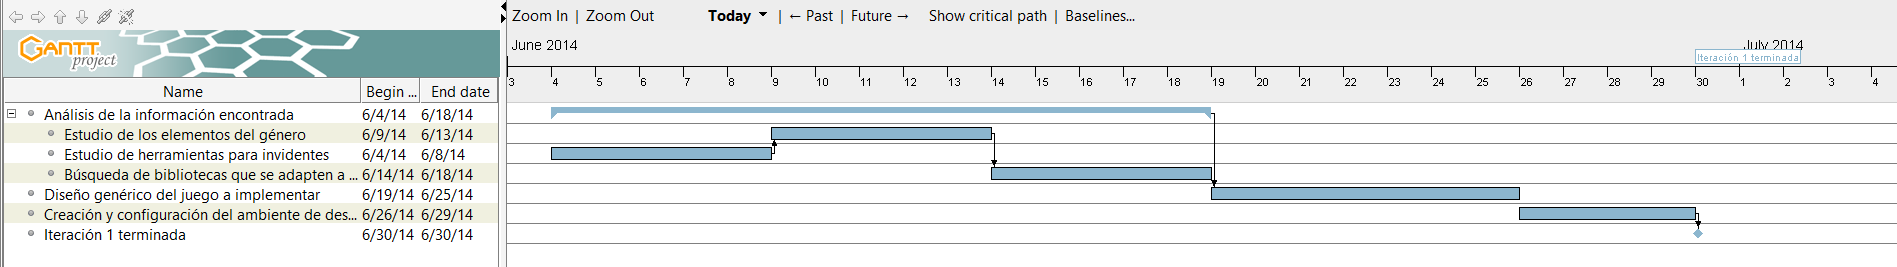
\includegraphics[width=\textwidth,height=\textheight,keepaspectratio]{./img/sec1it1.png}
  \caption{Diagrama de Gantt de la primera iteración de la primera etapa}
  \label{fig:sec1it1}
\end{figure}

\subsubsection{Qué hemos conseguido en esta iteración}

Comenzar un nuevo proyecto y recabar toda la información necesaria para tener una idea donde asentar las bases en las que se sembrarán las próximas iteraciones siempre es una tarea ardua y complicada. En esta iteración hemos sentado estas bases, definiendo lo que debemos de realizar y creando un primer boceto de lo que tendremos que cumplir durante los próximos meses.

\subsubsection{Qué queremos conseguir en la próxima iteración}

Con todo lo básico definido, ahora debemos de materalizarlo. Durante las siguientes iteraciones deberemos de empezar a crear el juego en sí, empezando por los mapas y habitaciones.

\subsection{Segunda iteración: Generación de mapas y habitaciones}

Desde el 15 de julio hasta el 24 de septiembre.

\paragraph{Análisis de requisitos de los mapas y habitaciones} Hay mucho escrito y realizado sobre la creación de mapas y habitaciones de forma aleatoria. En base toda esta información, debemos de elegir lo que queremos realizar en base a, por ejemplo, si el tamaño de dicho mapa siempre será el mismo o no, cómo y cuántas habitaciones queremos tener en cada mapa y el tipo de aletoriedad que queremos (completamente aleatorio o pseudo-aleatorio).

\paragraph{Diseño de los mapas y las habitaciones} Una vez hayamos creado el análisis de requisitos y tengamos toda la información necesaria sobre la mesa, es hora de crear el diseño. Dicho diseño debe de ser fácilmente extendible para que la realización de pequeños cambios no sean un gran reto.

\paragraph{Creación de tests que cubran lo analizado} Tal y como comentamos anteriormente, antes de ponernos con la programación, crearemos los tests que especifiquen y cumplan lo diseñado para, posteriormente, empezar con la codificación.

\paragraph{Implementación del diseño de mapas y habitaciones} Con el diseño y los tests creados, es hora de la implementación del código analizado y diseñado.

\subsubsection{Tareas y seguimiento}

La descomposición de las tareas es la siguiente:

\begin{enumerate}[label=\bfseries WBS 2.\arabic*]
  \item Análisis de requisitos de los mapas y habitaciones.
    \begin{enumerate}[label=\bfseries WBS 2.1.\arabic*]
      \item Estudio de diferentes algoritmos de creación aleatoria de mapas y habitaciones.
      \item Decisión sobre la estructura y tamaño a elegir en base al tipo del juego.
    \end{enumerate}
  \item Diseño de los mapas y las habitaciones.
  \item Creación de tests que cubran lo analizado.
  \item Implementación del diseño de mapas y habitaciones.
\end{enumerate}

Para la realización de esta segunda iteración se planificaron 125 horas en total. La estimación no fue correcta y no fuimos capaces de finalizar todo lo necesario, por lo que tuvimos que dejar la tarea de representar este mapa para la siguiente iteración. Ver la figura ~\ref{fig:sec1it2}

\begin{figure}
    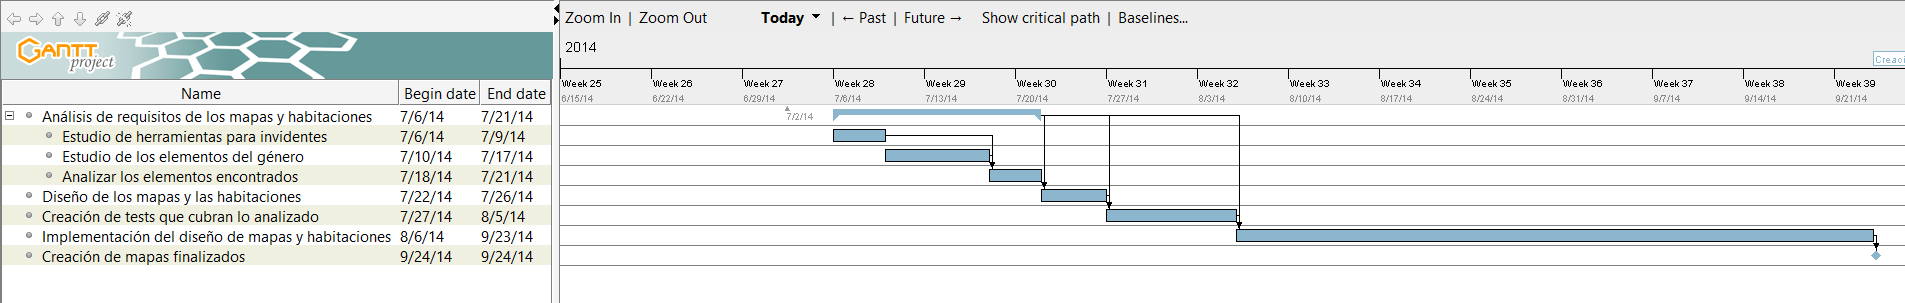
\includegraphics[width=\textwidth,height=\textheight,keepaspectratio]{./img/sec1it2.png}
  \caption{Diagrama de Gantt de la segunda iteración de la primera etapa}
  \label{fig:sec1it2}
\end{figure}

\subsubsection{Qué hemos conseguido en esta iteración}

Hemos conseguido generar mapas y habitaciones de manera aleatoria, pero todavía no mostrarlos en la interfaz de usuario. Uno de los puntos esenciales del género de los \textit{roguelike} es su aleatoriedad y conseguir que los mapas es el primer gran punto.

\subsubsection{Qué queremos conseguir en la próxima iteración}

En la siguiente iteración debemos de terminar lo que no hemos conseguido hacer en ésta, por lo que representar estos mapas en la interfaz gráfica toma prioridad. A continuación comenzaremos con la creación de objetos. Dichos objetos es otro de los puntos esenciales del género.

\section{Enero 2015 - Mayo 2015}

Este periodo comienza el 2 de enero, tras los días libres de navidad y nuevo año, y termina el 31 de mayo, en el que pararemos para preparar los exámenes. Por lo tanto, este periodo consta de un total de 21 semanas. Durante estas semanas he estado trabajando a tiempo completo y algunos días se los dediqué a estudiar para los exámenes, por lo que el tiempo semanal empleado fue de alrededor de 12 horas de media, aunque algunas de estas semanas fueron de más trabajo que otras.

En total, 170 horas fueron dedicadas para este sprint inicialmente.

Durante este sprint nos hemos centrado en continuar lo realizado anteriormente y, en general, seguir con el desarrollo del juego en sí.

\subsection{Primera iteración: mapas en IU, análisis, diseño, tests e implementación de los objetos}

Esta primera iteración comienza el 2 de enero y termina el 4 de marzo.

\paragraph{Mostrar los mapas y habitaciones en el interfaz de usuario} En la anterior fase implementamos los mapas, pero no los enseñamos en la interfaz de usuario. En esta ocasión debemos de acabar con esta tarea para terminar con todo lo relacionado con la creación de mapas.

\paragraph{Análisis de requisitos para sobre los objetos} En un \textit{roguelike} los objetos son primordiales. Debemos de investigar qué objetos vamos a usar y cómo los representaremos en el mapa diseñado anteriormente.

\paragraph{Crear un diseño simple sobre cómo los objetos interactuarán con el mapa} Debemos de crear un diseño genérico que nos permita añadir objetos de manera sencilla.

\paragraph{Creación de tests que cubran lo analizado} Al igual que antes, es necesario crear primero los tests en vez de empezar con la implementación del diseño directamente. En este caso también añadiremos tests que interactuen mapas y objetos para asegurarnos que no vamos a tener ningún error cuando combinemos ambos.

\paragraph{Implementación de los objetos en el juego} Una vez realizado el análisis, el diseño y los tests, podremos implementar la solución encontrada.

\subsubsection{Tareas y seguimiento}

La descomposición de las tareas es la siguiente:

\begin{enumerate}[label=\bfseries WBS 1.\arabic*]
  \item Mostrar los mapas y habitaciones en el interfaz de usuario.
  \item Análisis de requisitos sobre los objetos.
    \begin{enumerate}[label=\bfseries WBS 1.1.\arabic*]
      \item Buscar información sobre los diferentes tipos de objetos necesarios en el juego.
      \item Estudiar cómo estos objetos deben de interactuar con el mapa.
      \item Decidir y resumir lo encontrado.
    \end{enumerate}
  \item Crear un diseño simple sobre cómo los objetos interactuarán con el mapa.
  \item Creación de tests que cubran lo analizado.
  \item Implementación de los objetos en el juego y su asociación con el propio mapa y habitaciones.
\end{enumerate}

Para la realización de la primera iteración del segundo bloque de trabajo se planificaron 55 horas en total. La estimación fue correcta y fue posible cumplirla. Ver la figura ~\ref{fig:sec2it1}

\begin{figure}
    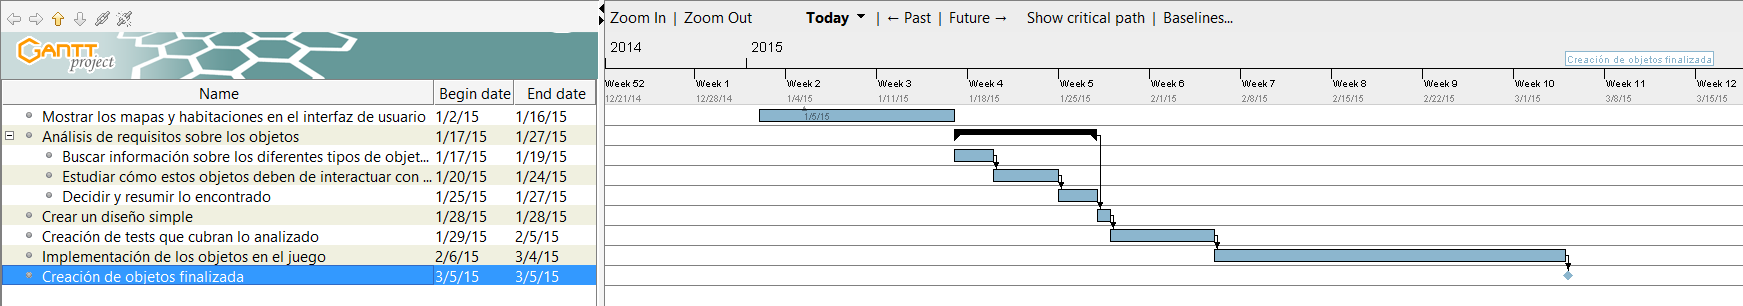
\includegraphics[width=\textwidth,height=\textheight,keepaspectratio]{./img/sec2it1.png}
  \caption{Diagrama de Gantt de la primera iteración de la segunda etapa}
  \label{fig:sec2it1}
\end{figure}

\subsubsection{Qué hemos conseguido en esta iteración}

Terminar la tarea restante del sprint anterior y la creación de diferentes objetos (pociones, armas y armaduras) que los personajes podrán utilizar. También podemos representar dichos objetos en el mapa, además de que la creación de nuevos elementos sea muy sencilla.

\subsubsection{Qué queremos conseguir en la próxima iteración}

Crear los personajes. Ésta es uno de los últimos pilares esenciales del género, por lo que tomará prioridad y será realizado a continuación.

\subsection{Segunda iteración: análisis, diseño, tests e implementación de los personajes}

La segunda iteración comienza el 5 de marzo y acaba el 23 de mayo.

\paragraph{Análisis de requisitos para sobre personajes} En el juego tendremos un personaje principal (controlado por el usuario) y una serie de enemigos con diferentes características que intentarán destruirle y que el usuario deberá de batir. En esta tarea nos encargaremos de buscar información sobre el tipo de enemigos a crear y diferentes métodos para hacerlo de forma más genérica posible, dado que ser capaz de crear estos enemigos fácilmente es una característica fundamental.

\paragraph{Creación del diseño de los personajes} Una vez hayamos realizado el análisis para obtener la idea de los enemigos y personajes a usar, es hora de crear el diseño. Tal y como hemos comentado anteriormente, es necesario hacer un diseño extendible donde crear diferentes clases de enemigos sea lo más sencillo posible.

\paragraph{Implementación de los tests} Como hasta ahora, antes de empezar con la implementación directamente, debemos de crear tests sobre ello, que nos indicará las características que deben de cumplir.

\paragraph{Programación de lo diseñado y analizado previamente} Con el análisis, diseño y tests listos, podremos realizar la tarea de implementación.

\subsubsection{Tareas y seguimiento}

La descomposición de las tareas es la siguiente:

\begin{enumerate}[label=\bfseries WBS 2.\arabic*]
  \item Análisis de requisitos sobre personajes (jugadores y enemigos)
    \begin{enumerate}[label=\bfseries WBS 2.1.\arabic*]
      \item Buscar información sobre los diferentes tipos de enemigos a los que nos enfrentaremos.
      \item Estudiar cómo estos enemigos interectuarán con el mapa y los objetos creados anteriormente.
      \item Decidir y resumir lo encontrado.
    \end{enumerate}
  \item Crear un diseño para crear, fácilmente, nuevos enemigos que aparezcan aleatoriamente en el mapa.
  \item Creación de tests que cubran lo analizado.
  \item Implementación de los enemigos en el juego y su asociación con el propio mapa, habitaciones y objetos.
\end{enumerate}

Para la realización de este \textit{sprint} se han asignado 80 horas, las cuales fueron suficientes para cubrir todo lo que se quiso realizar. Ver la figura ~\ref{fig:sec2it2}

\begin{figure}
    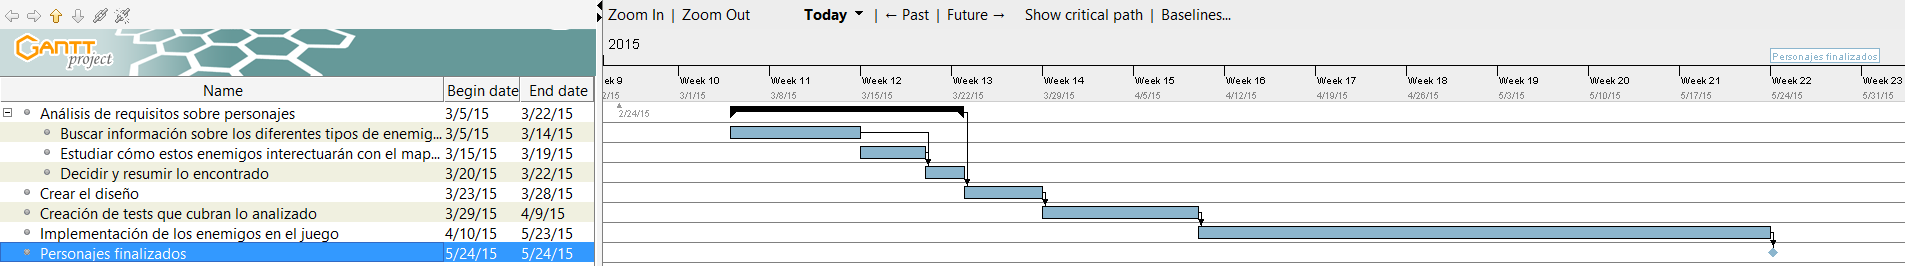
\includegraphics[width=\textwidth,height=\textheight,keepaspectratio]{./img/sec2it2.png}
  \caption{Diagrama de Gantt de la segunda iteración de la segunda etapa}
  \label{fig:sec2it2}
\end{figure}

\subsubsection{Qué hemos conseguido en esta iteración}

Al igual que con los objetos, hemos conseguido facilitar su creación, así como la representación del mapa de los mismos. Hemos creado un personaje principal (controlado por el usuario) y diferentes tipos de enemigos (doblins, ratas y dragones). Ambos tipos se muestran en el mapa.

\subsubsection{Qué queremos conseguir en la próxima iteración}

Tal y como tenemos el proyecto actualmente, tenemos el mapa creado aleatoriamente y podemos mostrar objetos y personajes con facilidad. El siguiente paso consiste en que los personajes puedan interactuar con los objetos.

\subsection{Tercera iteración: interacción entre personajes, tests e implementación}

Esta última iteración de la sección, y la más corta, comienza el 24 de mayo y acaba el 31 del mismo mes.

En la anterior iteración teníamos el objetivo de crear los personajes y enemigos y que éstos fueran capaces de ser representados en la interfaz gráfica. En este caso daremos un paso más allá y deberemos de añadir funciones que dichos personajes puedan realizar con los objetos: creación de un inventario para que puedan almacernarlos y, de tal modo, el usuario y enemigos puedan tener la habilidad de coger objetos (del mapa al inventario), tirarlos (del inventario al mapa), equiparlos (del inventario al personaje) y desequiparlos (del personaje al inventario).

\paragraph{Ampliar los tests sobre la interacción entre los objetos y personajes} En la iteración anterior fuimos capaces de crear los personajes de forma genérica y en este caso deberemos crear nuevas funciones que ayuden a la interacción entre los objetos y los personajes, tal y como hemos descrito anteriormente.

\paragraph{Implementación en base a los tests, análisis y diseño de la anterior iteración} El diseño y el análisis ya lo tenemos hecho y, una vez tengamos los tests creados, podremos realizar la implementación.

\subsubsection{Tareas y seguimiento}

La descomposición de las tareas es la siguiente:

\begin{enumerate}[label=\bfseries WBS 3.\arabic*]
  \item Ampliar los tests que tengan que ver con la interacción entre los objetos y personajes
  \item Implementación en base al diseño de la anterior iteración y los nuevos tests creados.
\end{enumerate}

\begin{figure}
    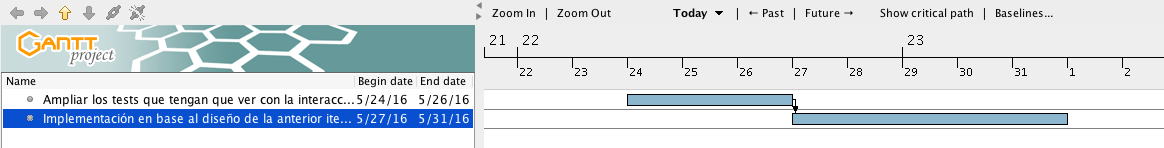
\includegraphics[width=\textwidth,height=\textheight,keepaspectratio]{./img/sec2it3.png}
  \caption{Diagrama de Gantt de la tercera iteración de la segunda etapa}
  \label{fig:sec2it3}
\end{figure}

Al ser un pequeño sprint, hemos sido capaces de terminarlo sin problema. El diagrama de Gantt puede verse en la figura ~\ref{fig:sec2it3}

\subsubsection{Qué hemos conseguido en esta iteración}

Interacción básica entre personajes y objetos.

\subsubsection{Qué queremos conseguir en la próxima iteración}

Aumentar esta interacción (que podamos atacar a los personaje, por ejemplo) y dar control al usuario, por lo que tendremos que diseñar la manera de que el usuario pueda decidir moverse, atacar, coger un objeto del mapa, etc.

\section{Septiembre 2015 - Abril 2016}

Este periodo empieza el 1 de septiembre, tras un breve descanso en verano, y termina el 31 de abril. Durante este tiempo hemos empleado más tiempo que anteriormente en el proyecto y desarrollado mucho más (20 horas a la semana). También hemos buscado \textit{feedback} una vez tuvimos tiempo disponible para poder tener tiempo para implementarlo y asegurarnos de que lo que hemos realizado es aceptado por la comunidad. 
Este periodo consta de un total de 34 semanas.

En total, 680 horas fueron dedicadas para este sprint inicialmente.

\subsection{Primera iteración: Aumentar interacción entre objetos, mapas y personajes, añadir movimiento para el jugador}

Esta primera iteración da comienzo el 1 de septiembre y acaba el 5 de octubre, es decir, damos 5 semanas para su realización.

\paragraph{Aumentar la interacción entre objetos, personajes y mapa} Hasta el momento tenemos el mapa, objetos y personajes, pero debemos de ser capaces de interactuar completamente y aumentar en características. Por ejemplo añadiendo puertas entre habitaciones, que también se muestren en el mapa, que los personajes puedan atacarse entre sí (teniendo en cuenta las armaduras y armas que llevan) y la creación de un campo de visión para el usuario para que solamente pueda ver lo que hay a su alrededor y no todo el mapa.

\paragraph{Agregar \textit{listeners} para que el jugador pueda decidir lo que hacer} En este momento el jugador no puede hacer nada. Ahora es el momento de introducir los elementos necesarios para que nos podamos mover por el mapa y realizar todas las acciones implementadas anteriormente con nuestro personaje.

\subsubsection{Tareas y seguimiento}

La descomposición de las tareas es la siguiente:

\begin{enumerate}[label=\bfseries WBS 1.\arabic*]
  \item Aumentar la interacción entre objetos, personajes y mapa.
    \begin{enumerate}[label=\bfseries WBS 1.1.\arabic*]
      \item Crear tests para los elementos posteriores
      \item Añadir puertas que unan las habitaciones para que el jugador pueda pasar de habitación a habitación.
      \item Añadir la posibilidad de ataque entre personajes.
      \item Añadir un campo de visión al usuario para que no sea capaz de ver todo el mapa, pero solamente cierta área a su alrededor.
    \end{enumerate}
  \item Agregar \textit{listeners} para que el jugador pueda decidir lo que hacer.
\end{enumerate}

Hemos asignado 100 horas para la estimación de este \textit{sprint}, las cuales cumplimos sin problema. Ver la figura ~\ref{fig:sec3it1}

\begin{figure}
    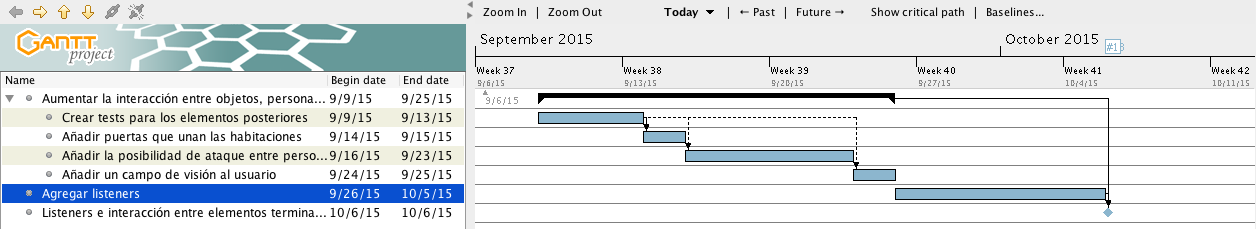
\includegraphics[width=\textwidth,height=\textheight,keepaspectratio]{./img/sec3it1.png}
  \caption{Diagrama de Gantt de la primera iteración de la tercera etapa}
  \label{fig:sec3it1}
\end{figure}

\subsubsection{Qué hemos conseguido en esta iteración}

Al acabar esta iteración tenemos lo básico de un juego: nos podemos mover por un mapa, coger objetos y combatir enemigos (aunque estos enemigos todavía no tienen inteligencia artificial, por lo que no se mueven).

\subsubsection{Qué queremos conseguir en la próxima iteración}

En la próxima iteración deberemos terminar lo básico del juego. Para ello tendremos que implementar el sistema de portales (que nos transportarán a un mapa completamente diferente, consiguiendo puntos de esta manera), añadir básica inteligencia artifial a los enemigos e incorporar la opción de cambiar el color de la interfaz de usuario para que se adapte a los jugadores daltónicos, tal y como hemos explicado en la sección \label{sec:daltonicossolventar}

\subsection{Segunda iteración: Diseño e implementación de los portales, IA de los enemigos y accesibilidad para daltónicos}

Esta segunda iteración comienza el 6 de octubre y termina el 8 de noviembre, con 4 semanas y media para su finalización.

\paragraph{Diseño e implementación de los portales} El sistema de portales fue la idea principal que tuvimos para crear un sistema de puntuación y progreso para el usuario. El objetivo está en encontrar el portal dentro del mapa y, una vez encontrado, un nuevo mapa será generado, igual que otro portal en ese mapa. De esta manera la meta del juego se centra en derrotar enemigos (consiguiendo mejores armas y armaduras en el proceso) para encontrar el mayor número de portales posibles.
Deberemos de diseñar e implementar estos portales en esta iteración.

\paragraph{Añadir inteligencia artificial} Dependiendo del enemigo al que nos enfrentemos, éste se comportará de forma distinta. Habrá enemigos que sean activos y vayan contra el usuario, mientras que otros serán pasivos y no quieran atacar al usuario. Puede ser que en el futuro queramos incrementar el número de este tipo de comportamientos, por lo que deberemos de diseñarlo de la mejor forma.

\paragraph{Añadir opciones para cambiar el color de la interfaz gráfica} El punto central de este proyecto es la accesibilidad e incluir una opción para que daltónicos puedan disfrutar de nuestro juego es decisivo.

\subsubsection{Tareas y seguimiento}

La descomposición de las tareas es la siguiente:

\begin{enumerate}[label=\bfseries WBS 2.\arabic*]
  \item Diseño e implementación de los portales.
    \begin{enumerate}[label=\bfseries WBS 2.1.\arabic*]
      \item Diseñar la mejor manera para incluir los portales en nuestro diseño (en el análisis es algo que se había considerado hacer).
      \item Creación de los tests.
      \item Implementación de los portales.
    \end{enumerate}
  \item Añadir inteligencia artificial.
  	\begin{enumerate}[label=\bfseries WBS 2.2.\arabic*]
      \item Diseñar la mejor manera para incluir diferentes tipos de IA.
      \item Crear los tests de IA.
      \item Implementar esta IA para los enemigos.
    \end{enumerate}
  \item Añadir opciones para cambiar el color de la interfaz gráfica para usuarios daltónicos
\end{enumerate}

48 horas fueron las que creímos suficientes para la estimación del \textit{sprint} y que fueron necesarias para la conclusión del mismo con todas las tareas terminadas. Ver la figura ~\ref{fig:sec3it2} como referencia.

\begin{figure}
    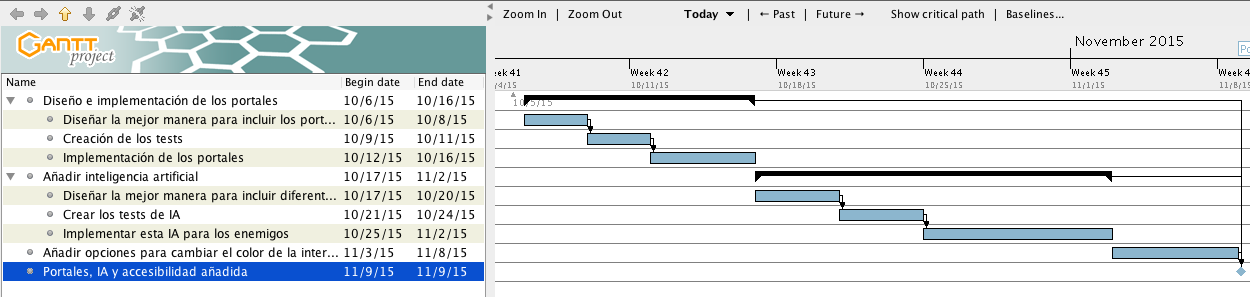
\includegraphics[width=\textwidth,height=\textheight,keepaspectratio]{./img/sec3it2.png}
  \caption{Diagrama de Gantt de la segunda iteración de la tercera etapa}
  \label{fig:sec3it2}
\end{figure}

\subsubsection{Qué hemos conseguido en esta iteración}

Con esta última iteración tenemos la parte básica del juego completada. Hay un objetivo, enemigos con IA, diferentes objetos, puertas que conectan distintas habitaciones y varias acciones que se pueden realizar.

\subsubsection{Qué queremos conseguir en la próxima iteración}

Con el juego en sí completado (o por lo menos la parte primordial), es hora de empezar a analizar y diseñar la parte de la generación automática del lenguaje.

\subsection{Tercera iteración: Análisis, diseño básico y comienzo de la implementación de las gramáticas}

Esta segunda iteración comienza el 9 de noviembre y termina el 31 de diciembre, con 6 semanas y media para su finalización.

\paragraph{Análisis de las gramáticas} Una parte muy importante del juego es crear frases que sean generadas de forma automática y pseudo-aleatoria en base a una serie de gramáticas y diccionario dado. Si conseguimos realizar esto, crear diferentes idiomas sería trivial (solamente tendríamos que cambiar la gramática en caso de que en dicho idioma sea diferente y traducir el diccionario). Para ello tendremos que investigar cómo podemos hacer esto en nuestro caso y cómo han solventado este problema otra gente.

\paragraph{Diseño general sobre la generación del lenguaje} Una vez hemos analizado y decidido lo que debemos de realizar, crearemos un diseño lo más simple y adaptable posible para la generación de dichas frases en base a las gramáticas dadas.

\paragraph{Creación de gramáticas y diccionarios base} Para empezar el desarrollo necesitamos tener una gramática y diccionaro base con lo que poder ver los diferentes resultados obtenidos.

\subsubsection{Tareas y seguimiento}

La descomposición de las tareas es la siguiente:

\begin{enumerate}[label=\bfseries WBS 3.\arabic*]
  \item Análisis de las gramáticas.
    \begin{enumerate}[label=\bfseries WBS 3.1.\arabic*]
      \item Leer la información que existe sobre la generación automática de lenguaje.
      \item Estudiar cómo lo podemos implementar en nuestro proyecto con lo ya existente.
      \item Tomar la decisión en base a lo encontrado y sentar las bases sobre ello.
    \end{enumerate}
  \item Diseño general sobre la generación del lenguaje y cómo las gramáticas interactuarán con nuestro programa.
  \item Creación de gramáticas y diccionarios base para tener una base con lo que testar lo que implementaremos.
\end{enumerate}

Hemos reservado 130 horas para esta iteración y hemos conseguido terminar todas las tareas asignadas a tiempo. Ver la figura ~\ref{fig:sec3it3} para más información.

\begin{figure}
    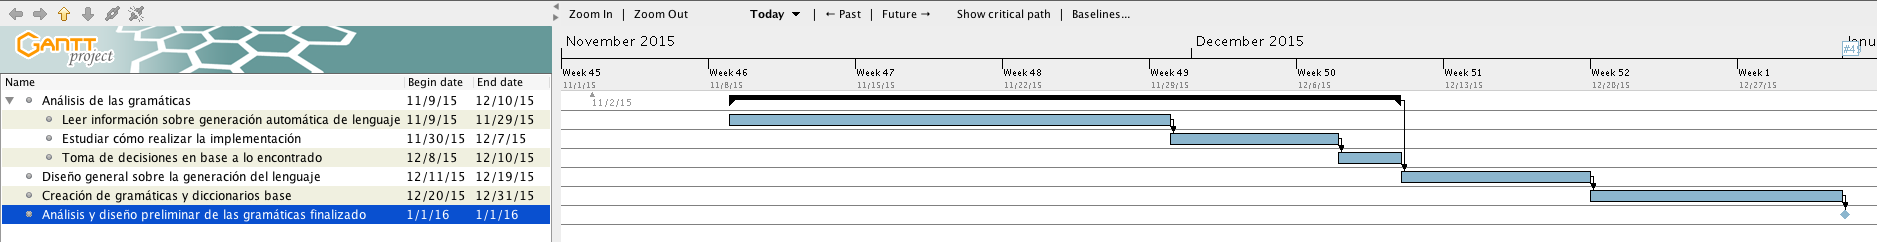
\includegraphics[width=\textwidth,height=\textheight,keepaspectratio]{./img/sec3it3.png}
  \caption{Diagrama de Gantt de la tercera iteración de la tercera etapa}
  \label{fig:sec3it3}
\end{figure}

\subsubsection{Qué hemos conseguido en esta iteración}

Hemos sentado las bases de lo que queremos implementar con las gramáticas.

\subsubsection{Qué queremos conseguir en la próxima iteración}

Empezar con los tests y desarrollo de lo investigado en esta iteración.

\subsection{Cuarta iteración: Análisis, diseño y comienzo de la implementación de las gramáticas}

Esta segunda iteración comienza el 1 de enero y termina el 19 de enero. Es decir, tiene 2 semanas y media de duración.

\paragraph{Análisis sobre cómo crear las gramáticas NP\footnote{\textit{noun phrase}. Sintagma nominal.} Las gramáticas NP son básicas, pero no iguales en todos los idiomas. Debemos de estudiar qué planteamientos existen que faciliten su implementación de la mejor forma posible.

\paragraph{Diseño de las gramáticas NP} Las frases de sintagma nominal serán las más usadas dentro de nuestro juego. No solamente serán utilizadas para la generación de las frases, pero también a la hora de representar los elementos en la interfaz de usuario. Por ello debemos de crearlas de la forma más extendible y accesible que podamos.

\paragraph{Creación de los tests para las gramáticas NP} Al igual que en otras iteraciones, realizamos los tests antes de nada.

\paragraph{Implementación de las gramáticas NP} Con los tests realizados, debemos de empezar con la implementación. Tenemos que tener en cuenta que hay que ser capaces de sustituir las clases de palabras por las palabras en sí que se encuentra en el diccionario. También hay que tener en cuenta las restricciones posibles (por el momento solamente contamos con las restricciones de inglés. Es decir, número).

\subsubsection{Tareas y seguimiento}

La descomposición de las tareas es la siguiente:

\begin{enumerate}[label=\bfseries WBS 4.\arabic*]
  \item Análisis sobre cómo crear las gramáticas NP de forma genérica y fácilmente extendibles para otros idiomas.
  \item Diseño de las gramáticas NP.
  \item Creación de los tests para las gramáticas NP.
  \item Implementación de las gramáticas NP y \textit{link} con el diccionario.
\end{enumerate}

Hemos reservado 50 horas para esta iteración y terminamos todas las tareas a tiempo. Ver la figura ~\ref{fig:sec3it4} para más información.

\begin{figure}
    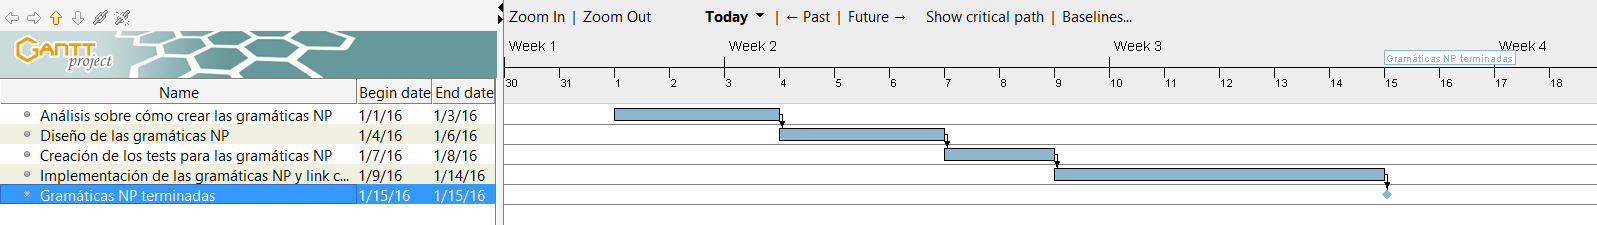
\includegraphics[width=\textwidth,height=\textheight,keepaspectratio]{./img/sec3it4.png}
  \caption{Diagrama de Gantt de la cuarta iteración de la tercera etapa}
  \label{fig:sec3it4}
\end{figure}

\subsubsection{Qué hemos conseguido en esta iteración}

Al finalizar esta iteración hemos conseguido generar sintagmas nominales de forma pseudo-aleatoria que basan su información en las gramáticas y diccionarios dados.

\subsubsection{Qué queremos conseguir en la próxima iteración}

Aumentar estas gramáticas para que lo generado no solamente sean sintagmas nominales, pero también frases que usen estos sintagmas nominales.

% Add restrictions for Spanish language in following sprints. Añadir UI para las gramáticas.